\documentclass[../main.tex]{subfiles}
\begin{document}

\chapter{Risultati}

\section{Metodi di valutazione}

Per misurare l'efficacia di questi filtri sono stati presi in considerazione diversi metodi di valutazione. La mancanza di immagini senza rumore di riferimento impedisce l'uso di metodi di valutazione full-reference (\acrshort{friqa}) ampiamente utilizzati, come \acrshort{psnr}\cite{korhonen_2012}, \acrshort{ssim}\cite{wang_2004} e \acrshort{cnr}.\cite{rodriguez_2018} La difficoltà nel valutare la qualità di queste immagini deriva anche dalla mancanza di valutazioni soggettive di esperti nel campo e dalla limitata quantità di letteratura su questo argomento.

In questo lavoro sono stati usati alcuni sistemi di valutazione cieca (\acrshort{nriqa}) basati su modelli statistici di immagini naturali, come \acrshort{brisque}\cite{mittal_2011}, \acrshort{niqe}\cite{mittal_2013} e \acrshort{piqe}\cite{venkatanath_2015}, usando i loro modelli predefiniti. Questi sistemi valutano la qualità dell'immagine con un punteggio da 0 in su, dove 0 corrisponde alla massima qualità. Oltre ai punteggi di questi modelli è stata misurata anche la variazione totale dell'immagine (\acrshort{tv}).

È stata inoltre condotta un'analisi correlativa tra le proprietà delle immagini di ampiezza \acrshort{snom} prese in esame e le corrispettive immagini di topografia \acrshort{afm}, in quanto questa immagine contiene una quantità di rumore molto inferiore rispetto alla prima.

\begin{figure}[ht]
	\centering
	\begin{subfigure}{0.4\linewidth}
		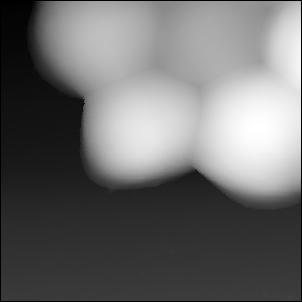
\includegraphics[keepaspectratio, width=\linewidth]{images/sa_zoom_z.png}
		\caption{Topografia \acrshort{afm}}
	\end{subfigure}\hspace{12pt}
	\begin{subfigure}{0.4425\linewidth}
		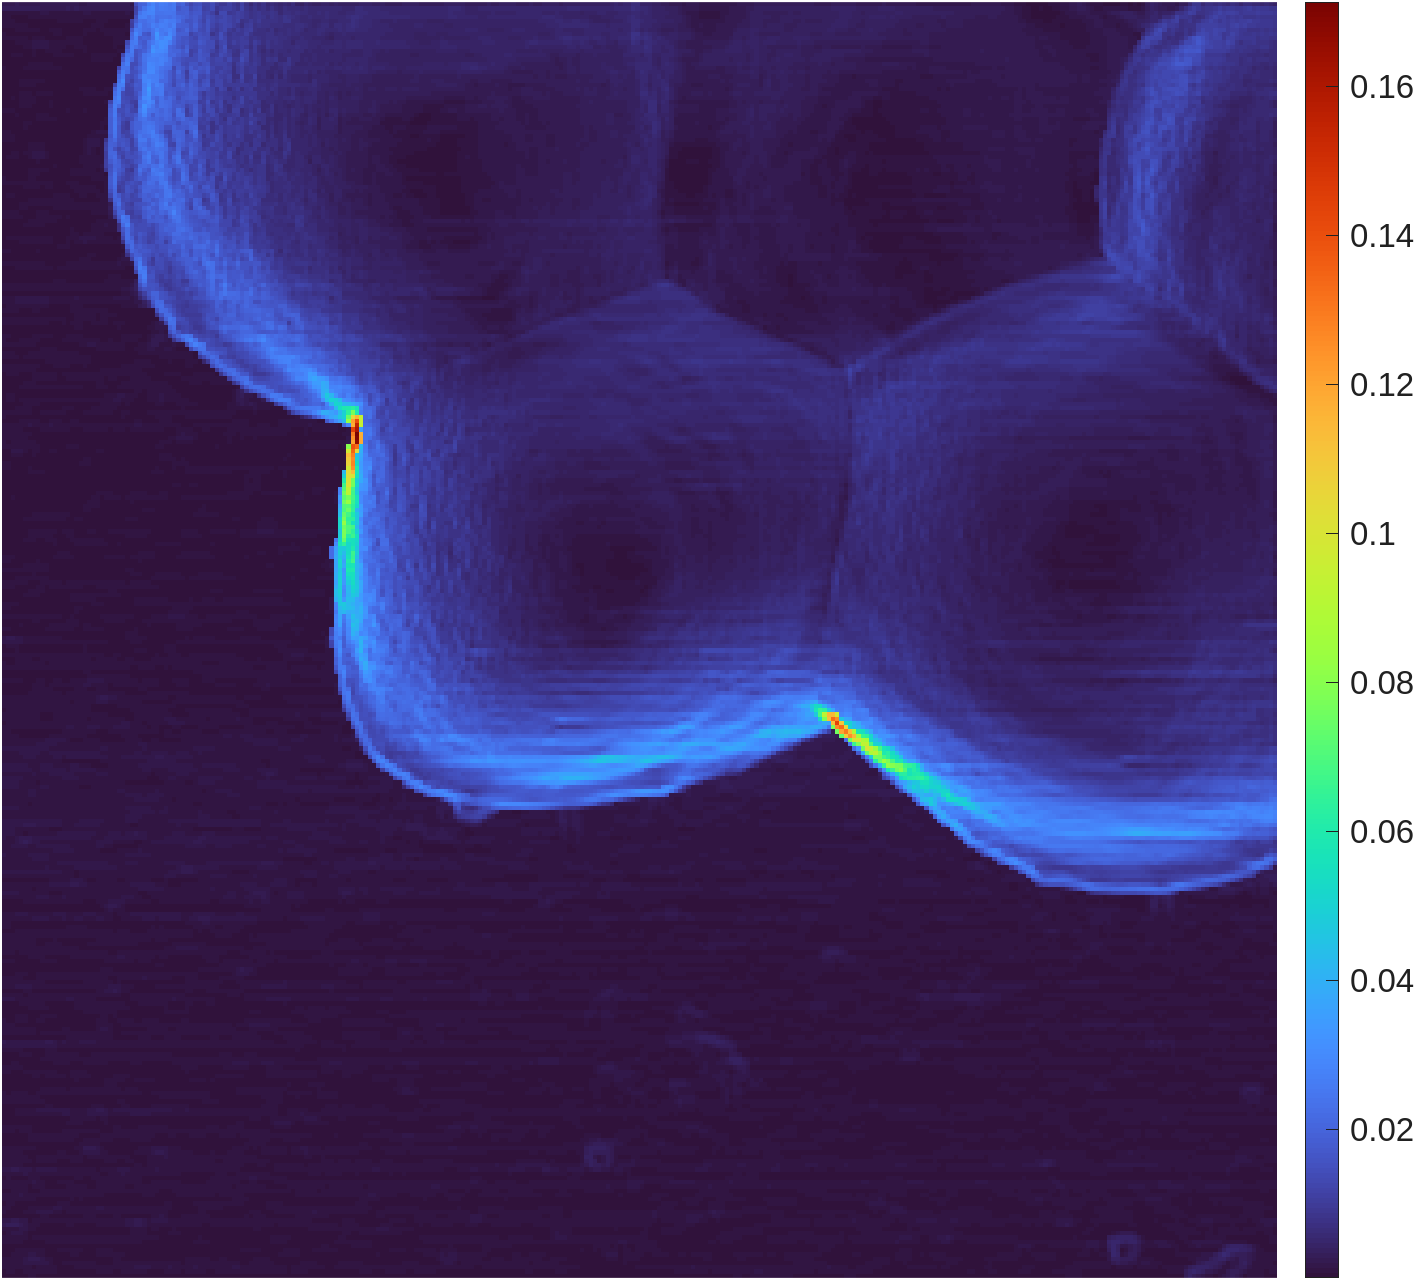
\includegraphics[keepaspectratio, width=\linewidth]{images/local_std_z.png}
		\caption{Deviazione standard topografia}
	\end{subfigure}\\[4pt]
	\begin{subfigure}{0.4\linewidth}
		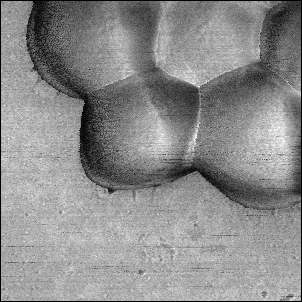
\includegraphics[keepaspectratio, width=\linewidth]{images/sa_zoom_o3a.png}
		\caption{Ampiezza \acrshort{ssnom} --- $3^a$ armonica}
	\end{subfigure}\hspace{12pt}
	\begin{subfigure}{0.4425\linewidth}
		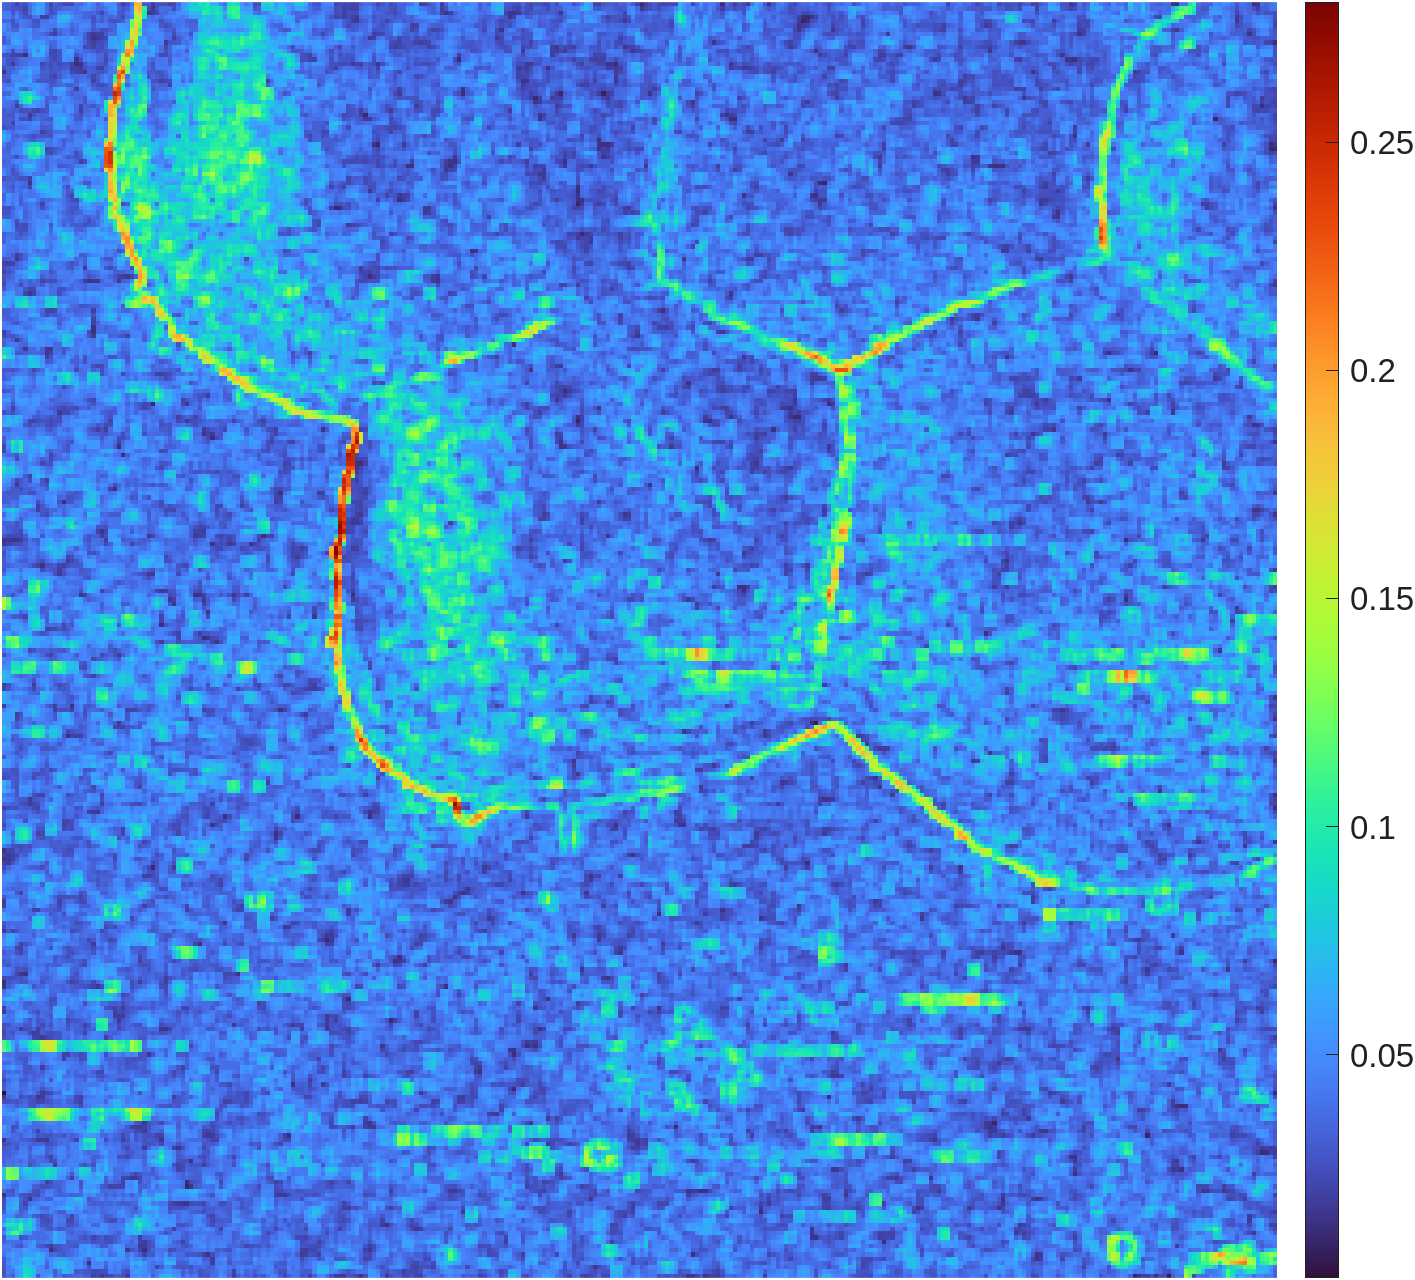
\includegraphics[keepaspectratio, width=\linewidth]{images/local_std_o3a.png}
		\caption{Deviazione standard ampiezza \acrshort{ssnom}}
	\end{subfigure}
	\caption[Confronto della deviazione standard locale tra immagini AFM e SNOM]{
		Confronto della deviazione standard locale tra immagini \acrshort{afm} e \acrshort{snom}}
\end{figure}

\subsection{Analisi correlativa}

Le immagini di topografia \acrshort{afm} e ampiezza \acrshort{snom}, anche se condividono delle informazioni spaziali correlate, non possono essere esaminate con i metodi di valutazione full-reference tradizionali poiché non rappresentano lo stesso contenuto. Le prime sono una mappa altimetrica del campione, mentre le seconde catturano le interazioni ottiche nel campo vicino, che dipendono dai materiali del campione.

Per svolgere questa analisi sono stati presi in considerazione cinque parametri:

\begin{enumerate}
	\itemsep0em
	\item Indice di Dice sui bordi
	\item Mutua informazione delle immagini
	\item Errore quadratico medio dell'entropia
	\item Congruenza di fase
	\item Modulo dei gradienti
\end{enumerate}

L'\textbf{indice di Dice} è usato per misurare la somiglianza tra due campioni studiando la presenza o assenza di elementi in comune, in questo caso la sovrapposizione tra l'immagine dei bordi della topografia e dell'ampiezza \acrshort{snom}. Un valore vicino a $1$ indica un'ottima sovrapposizione dei bordi mentre uno vicino a $0$ indica una scarsa sovrapposizione.\cite{carass_2020}

\begin{equation}
	S = 2\cdot \frac{\left|E_{X} \cap  E_{Y}\right|}{\left|E_{X}\right| + \left|E_{Y}\right|}
\end{equation}

La \textbf{mutua informazione} (\acrshort{mi}) è una misura statistica che quantifica quante informazioni una variabile contiene su un'altra, in questo caso un'immagine.\cite{shannon_1948} Questa misura è strettamente collegata al concetto di entropia di una variabile ed è ampiamente utilizzata nella correlazione e registrazione di immagini multimodale in cui vengono confrontati due diversi tipi di immagini,\cite{viola_1997} ad esempio RM e TAC,\cite{mclaughlin_2004, veninga_2004} usata in questo caso su \acrshort{afm} e \acrshort{ssnom}. La mutua informazione è nulla se $X$ e $Y$ sono variabili indipendenti.
\begin{equation}
	\begin{aligned}
		I(X,Y)  &= \sum_{x\in X}\sum_{y\in Y} p(x,y) \log\left(\frac{p(x,y)}{p_1(x)p_2(y)}\right) =\\
		&= H(X) + H(Y) - H(X,Y)
	\end{aligned}
\end{equation}

L'\textbf{entropia} è una misura della complessità spaziale dell'immagine, per cui regioni con un'alta entropia presentano strutture fine, texture o bordi marcati mentre regioni con un'entropia bassa presentano superfici lisce o uniformi. Ricavando l'errore quadratico medio dell'entropia rispetto all'immagine di topografia si può stimare la differenza di dettagli o rumore tra le due. Se l'errore è piccolo allora le due immagini avranno complessità spaziale simile negli stessi punti, mentre se è alto le strutture locali saranno differenti.
\begin{equation}
	\text{MSE} = \frac{1}{N}\sum_{i\in\Omega}\left(H_1(i)-H_2(i)\right)^2
\end{equation}

Un'altra misura per la stima delle strutture locali è la \textbf{congruenza di fase} (\acrlong{pc} --- \acrshort{pc}), secondo la quale le caratteristiche sono percepite in punti in cui le componenti di Fourier sono massime in fase. La congruenza di fase fornisce un modello semplice ma biologicamente plausibile di come il sistema visivo umano rileva e identifica le caratteristiche di un'immagine.\cite{kovesi_1999,morrone_1988}

Nel caso di segnali unidimensionali, questi si possono scomporre in $N$ componenti armoniche con ampiezza locale $A_n(x)$ e fase locale $\phi_n(x)$. La congruenza di fase nella posizione $x$ sarà il massimo allineamento di queste fasi. Quando tutte le fasi sono allineate, i termini del coseno valgono $1$ e di conseguenza si avrà $\text{PC} = 1$, mentre quando sono casuali il numeratore tende a $0$.
\begin{align}
	\text{PC}(x) &= \underset{\bar{\phi}(x)}{\max}\frac{\sum_n A_n(x) \cos\left(\phi_n(x) - \bar{\phi}(x)\right)}{\sum_n A_n(x)}\\[10pt]
	\bar{\phi}(x) &= \tan^{-1}\left(\frac{\sum_n A_n(x)\sin\phi_n(x)}{\sum_n A_n(x)\cos\phi_n(x)}\right)
\end{align}

Questo metodo non può essere usato per segnali bidimensionali come le immagini perché la trasformata di Hilbert non è definita per spazi multidimensionali e la trasformata di Fourier non è adatta a localizzare spazialmente le informazioni in frequenza. I sistemi moderni utilizzano una banca di filtri log-Gabor in diverse scale spaziali $s$ e orientamenti $o$ per misurare la congruenza di fase. Questo è implementato con delle paia di filtri in quadratura, in cui uno è pari $M^e_{s,o}$ e l'altro è dispari $M^o_{s,o}$.\cite{kovesi_2003}
\begin{align}
	\text{PC}(\mathbf{x}) &= \frac{\sum_o \mathcal{E}_o(\mathbf{x}) - T_o}{\sum_o\sum_s A_{s,o}(\mathbf{x})+\varepsilon}\\[6pt]
	\mathcal{E}_o(\mathbf{x}) &= \sqrt{\left(\sum_s I(\mathbf{x}) * M^e_{s,o}\right)^2 + \left(\sum_s I(\mathbf{x}) * M^o_{s,o}\right)^2}\\[6pt]
	A_{s,o}(\mathbf{x}) &= \sqrt{\left(I(\mathbf{x}) * M^e_{s,o}\right)^2 + \left(I(\mathbf{x}) * M^o_{s,o}\right)^2}
\end{align}

la congruenza di fase è combinata con l'\textbf{ampiezza dei gradienti} per formare l'indice \acrshort{fsim}, usato per misurare la similarità strutturale di due immagini in modo indipendente dall'intensità delle immagini.\cite{zhang_2011} Per calcolare i gradienti è usato l'operatore di Scharr.\cite{jahne_1999}
\begin{equation}
	G_x(\mathbf{x}) = \frac{1}{16}\begin{bmatrix}
		3 & 0 & -3 \\
		10 & 0 & -10 \\
		3 & 0 & -3
	\end{bmatrix} * I(\mathbf{x}) \qquad
	G_y(\mathbf{x}) = \frac{1}{16}\begin{bmatrix}
		3 & 10 & 3 \\
		0 & 0 & 0 \\
		-3 & -10 & 3 
	\end{bmatrix} * I(\mathbf{x})
\end{equation}

\newpage

\section{Discussione}

Dopo aver applicato le varie tecniche di riduzione del rumore alle immagini e aver registrato i corrispondenti parametri di valutazione, si è calcolata la media di questi ultimi. Nei metodi che richiedono una stima del rumore nell'immagine o un grado di smussamento è stata calcolata una stima 

Si può notare come nei metodi di valutazione \acrshort{nriqa} (\acrshort{brisque}, \acrshort{niqe} e \acrshort{piqe}) il filtro mediana sia quello che ricopre la posizione migliore, posizionandosi sempre al primo posto nelle immagini O3A e per due volte su tre anche per le immagini O2A. 

\begin{table}[h]
	\centering
	\begin{tabular}{l||ccc||ccc}
					  & \multicolumn{3}{c||}{O2A} & \multicolumn{3}{c}{O3A} \\
		              & BRISQUE & NIQE & PIQE     & BRISQUE & NIQE  & PIQE\\ \hline\hline
		Orignale      & 31.028 & 10.772 & 35.952  & 37.379 & 13.056 & 48.455 \\
		NLM           & 37.419 & 7.667 & 45.094   & 28.716 & 6.902  & 31.237 \\
		Mediana       & 30.333 & \textbf{4.595} & \textbf{25.323}   & \textbf{27.523} & \textbf{4.687}  & \textbf{19.609} \\
		Bilaterale    & 40.636 & 6.795 & 43.191   & 38.086 & 7.635  & 37.005 \\
		Wiener        & 35.567 & 5.533 & 32.181   & 34.382 & 5.458  & 22.755 \\
		Gaussiana 0.5 & \textbf{25.242} & 5.354 & 26.117   & 28.557 & 5.777  & 35.061 \\
		Gaussiana 2   & \textcolor{blue}{\textbf{55.467}} & 6.926 & \textcolor{blue}{\textbf{93.068}}   & \textcolor{blue}{\textbf{56.564}} & 6.814  & \textcolor{blue}{\textbf{90.359}} \\
		Rettangolare  & 34.036 & 4.702 & 30.313   & 33.615 & 4.785  & 21.585 \\
		Guidato       & \textcolor{blue}{\textbf{56.846}} & 6.612 & \textcolor{blue}{\textbf{89.204}}   & \textcolor{blue}{\textbf{57.741}} & 6.553  & \textcolor{blue}{\textbf{87.870}} \\
		BM3D          & 38.528 & 6.532 & 46.523   & 35.214 & 5.591  & 41.416
	\end{tabular}
	\caption[Valori medi dei metodi di valutazione NR-IQA]{
		Valori medi dei metodi di valutazione \acrshort{nriqa}}
\end{table}

Questo comportamento deriva dal fatto che il filtro mediana è un buon filtro da utilizzare per rimuovere i rumori di tipo impulsivo, che sono presenti in queste immagini e sono riconosciuti dai modelli di valutazione.\medskip

\begin{figure}[ht]
	\centering
	\begin{subfigure}{0.35\linewidth}
		\centering
		\begin{tikzpicture}
			\begin{scope}[
				node distance = 11mm,
				inner sep = 0pt,spy using outlines={rectangle, red, magnification=6}]
				\node (n0)  {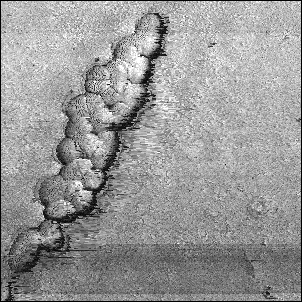
\includegraphics[keepaspectratio,width=\linewidth]{images/ef_o2a_orig.png}};
				
				\spy [white,size=1.5cm] on (-0.825,1.175) in node[below right=of n0.center];
			\end{scope}
			\draw[dashed,white] (tikzspyonnode.north east) -- (tikzspyinnode.north east);
			\draw[dashed,white] (tikzspyonnode.south west) -- (tikzspyinnode.south west);
		\end{tikzpicture}
		\caption{Originale}
	\end{subfigure}
	\hspace{10pt}
	\begin{subfigure}{0.35\linewidth}
	\centering
	\begin{tikzpicture}
		\begin{scope}[
			node distance = 11mm,
			inner sep = 0pt,spy using outlines={rectangle, red, magnification=6}]
			\node (n0)  {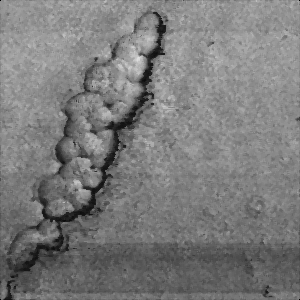
\includegraphics[keepaspectratio,width=\linewidth]{images/ef_o2a_med.png}};
			
			\spy [white,size=1.5cm] on (-0.825,1.175) in node[below right=of n0.center];
		\end{scope}
		\draw[dashed,white] (tikzspyonnode.north east) -- (tikzspyinnode.north east);
		\draw[dashed,white] (tikzspyonnode.south west) -- (tikzspyinnode.south west);
	\end{tikzpicture}
	\caption{Filtro mediana applicato}
	\end{subfigure}
	\caption{Immagine O3A con molto rumore impulsivo}
	\label{fig:ef1}
\end{figure}

In blu invece sono evidenziati gli outlier nella tabella: il filtro guidato e il filtro gaussiano con $\sigma = 2$. Questi filtri presentano dei valori di media in \acrshort{brisque} e \acrshort{piqe} molto superiori rispetto a tutti gli altri filtri esaminati. Questo si può notare anche nei valori medi della variazione totale, dove questi due filtri hanno ha media molto minore degli altri filtri.

\begin{table}[h]
	\centering
	\begin{tabular}{r||c|c}
		TV\hspace{10pt}	& O2A  & O3A \\\hline\hline
		Orignale   		& 4876 & 7594\\
		NLM         	& 2129 & 2010\\
		Mediana     	& 1585 & 2359\\
		Bilaterale    	& 2236 & 3832\\
		Wiener        	& 2112 & 2777\\
		Gaussiana 0.5 	& 2996 & 4532\\
		Gaussiana 2   	& \textcolor{blue}{\textbf{614}}  & \textcolor{blue}{\textbf{753}}\\
		Rettangolare 	& \textbf{1447} & \textbf{2006}\\
		Guidato        	& \textcolor{blue}{\textbf{610}}  & \textcolor{blue}{\textbf{742}}\\
		BM3D   			& 2072 & 2019
	\end{tabular}
	\caption{Valori medi della variazione totale}
\end{table}

Il filtro guassiano ad alta varianza smussa eccessivamente l'immagine, facendo perdere troppi dettagli e rendendo i bordi smussati. Anche il filtro guidato, avendo usato l'immagine della topografia come guida, visto che ha una varianta molto minore dell'immagine di ampiezza \acrshort{snom}, smussa eccessivamente le immagini. In conclusione, questi filtri sono stati scartati dalla valutazione.\\

\begin{figure}[ht]
	\centering
		\begin{subfigure}{0.45\linewidth}
		\centering
		\begin{tikzpicture}
			\begin{scope}[
				node distance = 6.5mm,
				inner sep = 0pt,spy using outlines={rectangle, red, magnification=6}]
				\node (n0)  {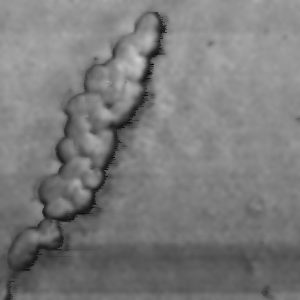
\includegraphics[keepaspectratio,width=\linewidth]{images/ef_o2a_guided.png}};
				
				\spy [white,size=2cm] on (-1.2,1.3) in node[below right=of n0.center];
			\end{scope}
			\draw[dashed,white] (tikzspyonnode.north east) -- (tikzspyinnode.north east);
			\draw[dashed,white] (tikzspyonnode.south west) -- (tikzspyinnode.south west);
		\end{tikzpicture}
		\caption{Filtro guidato}
	\end{subfigure}
	\hspace{10pt}
	\begin{subfigure}{0.45\linewidth}
		\centering
		\begin{tikzpicture}
			\begin{scope}[
				node distance = 6.5mm,
				inner sep = 0pt,spy using outlines={rectangle, red, magnification=6}]
				\node (n0)  {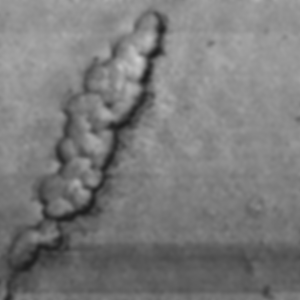
\includegraphics[keepaspectratio,width=\linewidth]{images/ef_o2a_gauss.png}};
				
				\spy [white,size=2cm] on (-1.2,1.3) in node[below right=of n0.center];
			\end{scope}
			\draw[dashed,white] (tikzspyonnode.north east) -- (tikzspyinnode.north east);
			\draw[dashed,white] (tikzspyonnode.south west) -- (tikzspyinnode.south west);
		\end{tikzpicture}
		\caption{Filtro gaussiano}
	\end{subfigure}
	\caption{Immagine della figura \ref{fig:ef1} elaborata con filtro gaussiano e guidato}
\end{figure}


Dalla valutazione è stata esclusa la scala \acrshort{fsim} in quanto non si possono apprezzare delle variazioni significative dei valori medi. Sono visibili anche in questa tabella i valori dei filtri outlier scartatati, a dimostrazione che l'ispezione visiva è uno step importante per la validazione dei risultati, in mancanza di un riferimento.\medskip

\begin{table}[ht]
	\centering
	\begin{tabular}{r||cc|cc}
		&  \multicolumn{2}{c|}{O2A} &  \multicolumn{2}{c}{O3A}  \\
		\acrshort{fsim}\hspace{10pt} & Valore & Diff & Valore & Diff \\		\hline\hline
		Orignale   		& 0.963 & ---   & 0.957 & --- \\
		NLM         	& 0.963 & 0     & 0.964 & 0.007 \\
		Mediana     	& 0.972 & 0.009 & 0.972 & 0.015 \\
		Bilaterale    	& 0.970 & 0.007 & 0.967 & 0.010 \\
		Wiener        	& 0.971 & 0.008 & 0.970 & 0.013 \\
		Gaussiana 0.5 	& 0.968 & 0.005 & 0.963 & 0.006 \\
		Gaussiana 2   	& \textcolor{blue}{\textbf{0.982}} & \textcolor{blue}{\textbf{0.019}} & \textcolor{blue}{\textbf{0.982}} & \textcolor{blue}{\textbf{0.025}} \\
		Rettangolare 	& \textbf{0.975} & \textbf{0.012} & \textbf{0.975} & \textbf{0.018} \\
		Guidato        	& \textcolor{blue}{\textbf{0.982}} & \textcolor{blue}{\textbf{0.019}} & \textcolor{blue}{\textbf{0.983}} & \textcolor{blue}{\textbf{0.026}} \\
		BM3D   			& 0.963 & 0     & 0.964 & 0.007	
	\end{tabular}
	\caption[Valori medi della scala FSIM]{
		Valori medi della scala \acrshort{fsim}}
\end{table}

Il filtro rettangolare si posiziona al primo posto sia nelle tabelle della variazione totale che in quelle della scala \acrshort{fsim}, con il filtro mediana che segue in seconda posizione con valori simili. I due filtri producono immagini con una quantità simile di rumore bianco sul piano di osservazione ma presentano dei comportamenti molto diversi in corrispondenza di regioni con variazioni di intensità elevate.\medskip

\begin{figure}[ht]
	\centering
	\begin{subfigure}{0.45\linewidth}
		\centering
		\begin{tikzpicture}
			\begin{scope}[
				node distance = 6.5mm,
				inner sep = 0pt,spy using outlines={rectangle, red, magnification=6}]
				\node (n0)  {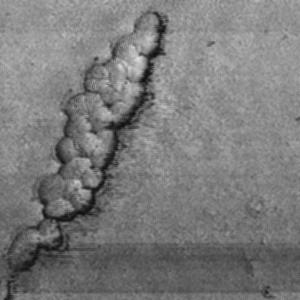
\includegraphics[keepaspectratio,width=\linewidth]{images/ef_o2a_box.png}};
				
				\spy [white,size=2cm] on (-1.2,1.3) in node[below right=of n0.center];
			\end{scope}
			\draw[dashed,white] (tikzspyonnode.north east) -- (tikzspyinnode.north east);
			\draw[dashed,white] (tikzspyonnode.south west) -- (tikzspyinnode.south west);
		\end{tikzpicture}
		\caption{Filtro rettangolare}
	\end{subfigure}
	\hspace{10pt}
	\begin{subfigure}{0.45\linewidth}
		\centering
		\begin{tikzpicture}
			\begin{scope}[
				node distance = 6.5mm,
				inner sep = 0pt,spy using outlines={rectangle, red, magnification=6}]
				\node (n0)  {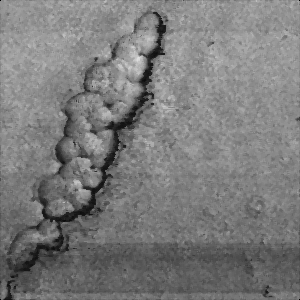
\includegraphics[keepaspectratio,width=\linewidth]{images/ef_o2a_med.png}};
				
				\spy [white,size=2cm] on (-1.2,1.3) in node[below right=of n0.center];
			\end{scope}
			\draw[dashed,white] (tikzspyonnode.north east) -- (tikzspyinnode.north east);
			\draw[dashed,white] (tikzspyonnode.south west) -- (tikzspyinnode.south west);
		\end{tikzpicture}
		\caption{Filtro mediana}
	\end{subfigure}
	\caption{Confronto tra filtro rettangolare e mediana}
	\label{fig:ef_bm}
\end{figure}

Il filtro mediana elimina le variazioni isolate e trasforma i bordi in gradini definiti, mentre si può notare come il filtro rettangolare generi degli artefatti nelle regioni dove prima era presente del rumore impulsivo, come si può osservare dalle striscie verticali e orizzontali presenti nella figura \ref{fig:ef_bm} in corrispondenza del rumore.

Passando agli ultimi metodi di valutazione che confrontano le caratteristiche dell'immagine di ampiezza \acrshort{snom} con quelle della topografia \acrshort{afm}, quindi la mutua informazione, l'indice di Dice sui bordi e l'errore quadratico medio dell'entropia, si può notare come, senza tener conto dei filtri scartati, i filtri che hanno avuto la performance migliori siano il filtro a media non locale e il filtro \acrshort{bm3d}.\medskip

\begin{table}[ht]
	\centering
	\begin{tabular}{r||ccc||ccc}
		& \multicolumn{3}{c||}{O2A} & \multicolumn{3}{c}{O3A} \\
		& EMSE & EDK & MI & EMSE & EDK & MI \\
		\hline\hline
		ORIGINAL     & 0.047 & 0.108 & 0.620 & 0.079 & 0.102 & 0.554 \\
		NLM          & 0.039 & \textbf{0.123} & \textbf{0.879} & \textbf{0.042} & \textbf{0.121} & \textbf{0.845} \\
		MEDIAN       & 0.044 & 0.114 & 0.738 & 0.056 & 0.106 & 0.706 \\
		BILAT        & 0.042 & 0.111 & 0.724 & 0.056 & 0.107 & 0.644 \\
		WIENER       & \textbf{0.037} & 0.111 & 0.717 & 0.043 & 0.107 & 0.660 \\
		GAUSSIAN 0.5 & 0.038 & 0.107 & 0.676 & 0.053 & 0.103 & 0.612 \\
		GAUSSIAN 2   & \textcolor{blue}{\textbf{0.045}} & \textcolor{blue}{\textbf{0.090}} & \textcolor{blue}{\textbf{0.885}} & \textcolor{blue}{\textbf{0.051}} & \textcolor{blue}{\textbf{0.093}} & \textcolor{blue}{\textbf{0.843}} \\
		AVERAGE      & 0.040 & 0.105 & 0.767 & 0.044 & 0.102 & 0.710 \\
		GUIDED       & \textcolor{blue}{\textbf{0.044}} & \textcolor{blue}{\textbf{0.105}} & \textcolor{blue}{\textbf{0.891}} & \textcolor{blue}{\textbf{0.049}} & \textcolor{blue}{\textbf{0.109}} & \textcolor{blue}{\textbf{0.853}} \\
		BM3D         & 0.047 & \textbf{0.121} & \textbf{0.845} & 0.063 & \textbf{0.119} & \textbf{0.827}
	\end{tabular}
	\caption{Valori medi dei metodi di valutazione correlativa}
\end{table}

\begin{figure}[ht]
	\centering
	\begin{subfigure}{0.45\linewidth}
		\centering
		\begin{tikzpicture}
			\begin{scope}[
				node distance = 6.5mm,
				inner sep = 0pt,spy using outlines={rectangle, red, magnification=6}]
				\node (n0)  {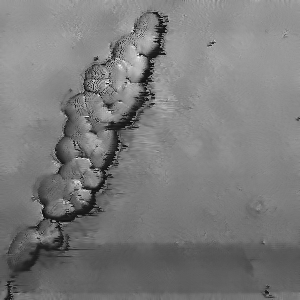
\includegraphics[keepaspectratio,width=\linewidth]{images/ef_o2a_nlm.png}};
				
				\spy [white,size=2cm] on (-1.2,1.3) in node[below right=of n0.center];
			\end{scope}
			\draw[dashed,white] (tikzspyonnode.north east) -- (tikzspyinnode.north east);
			\draw[dashed,white] (tikzspyonnode.south west) -- (tikzspyinnode.south west);
		\end{tikzpicture}
		\caption{Filtro \acrshort{nlm}}
	\end{subfigure}
	\hspace{10pt}
	\begin{subfigure}{0.45\linewidth}
		\centering
		\begin{tikzpicture}
			\begin{scope}[
				node distance = 6.5mm,
				inner sep = 0pt,spy using outlines={rectangle, red, magnification=6}]
				\node (n0)  {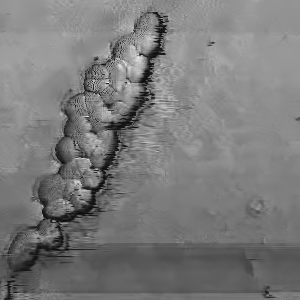
\includegraphics[keepaspectratio,width=\linewidth]{images/ef_o2a_bm3d.png}};
				
				\spy [white,size=2cm] on (-1.2,1.3) in node[below right=of n0.center];
			\end{scope}
			\draw[dashed,white] (tikzspyonnode.north east) -- (tikzspyinnode.north east);
			\draw[dashed,white] (tikzspyonnode.south west) -- (tikzspyinnode.south west);
		\end{tikzpicture}
		\caption{Filtro \acrshort{bm3d}}
	\end{subfigure}
	\caption[Confronto tra filtro NLM e BM3D]{
		Confronto tra filtro \acrshort{nlm} e \acrshort{bm3d}}
	\label{fig:ef_nlm}
\end{figure}

Questi filtri si basano entrambi sulla metodologia a media non locale e questo si nota soprattutto sulla grande differenza della varianza del rumore sullo sfondo, mantenendo però inalterate le strutture dei campioni. 

% concludi

\newpage
\null
\vfill
\begin{figure}[!ht]
	\centering
	\begin{subfigure}{0.3\linewidth}
		\centering
		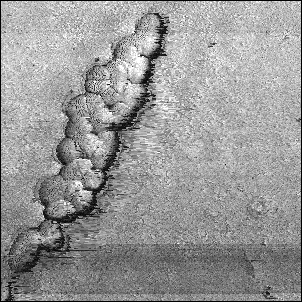
\includegraphics[keepaspectratio, width=\linewidth]{images/ef_o2a_orig.png}
	\end{subfigure}
	\hfill
	\begin{subfigure}{0.3\linewidth}
		\centering
		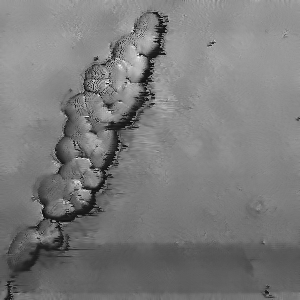
\includegraphics[keepaspectratio, width=\linewidth]{images/ef_o2a_nlm.png}
	\end{subfigure}
	\hfill
	\begin{subfigure}{0.3\linewidth}
		\centering
		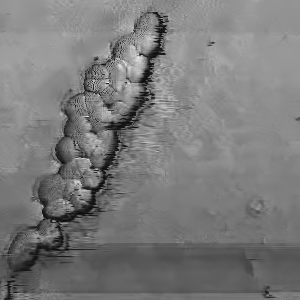
\includegraphics[keepaspectratio, width=\linewidth]{images/ef_o2a_bm3d.png}
	\end{subfigure}\\[20pt]
	\begin{subfigure}{0.3\linewidth}
		\centering
		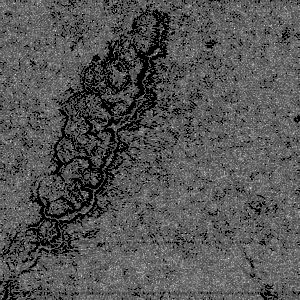
\includegraphics[keepaspectratio, width=\linewidth]{images/orig_grad.png}
	\end{subfigure}
	\hfill
	\begin{subfigure}{0.3\linewidth}
		\centering
		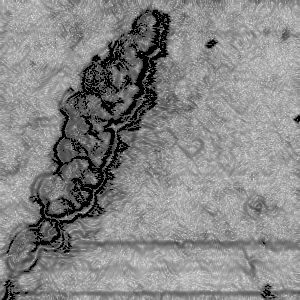
\includegraphics[keepaspectratio, width=\linewidth]{images/nlm_grad.png}
	\end{subfigure}
	\hfill
	\begin{subfigure}{0.3\linewidth}
		\centering
		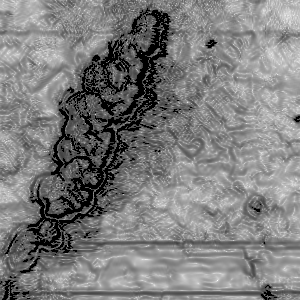
\includegraphics[keepaspectratio, width=\linewidth]{images/bm3d_grad.png}
	\end{subfigure}\\[20pt]
	\begin{subfigure}{0.3\linewidth}
		\centering
		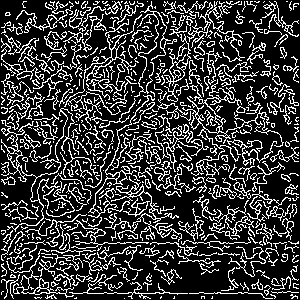
\includegraphics[keepaspectratio, width=\linewidth]{images/orig_edge.png}
	\end{subfigure}
	\hfill
	\begin{subfigure}{0.3\linewidth}
		\centering
		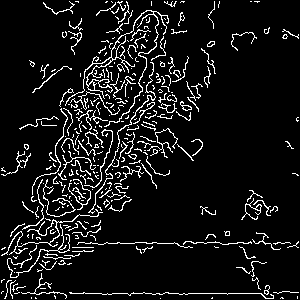
\includegraphics[keepaspectratio, width=\linewidth]{images/nlm_edge.png}
	\end{subfigure}
	\hfill
	\begin{subfigure}{0.3\linewidth}
		\centering
		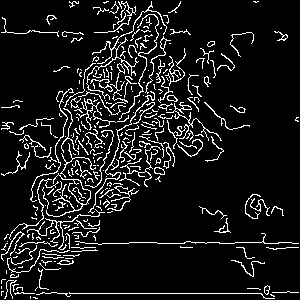
\includegraphics[keepaspectratio, width=\linewidth]{images/bm3d_edge.png}
	\end{subfigure}\\[20pt]
	\begin{subfigure}{0.3\linewidth}
		\centering
		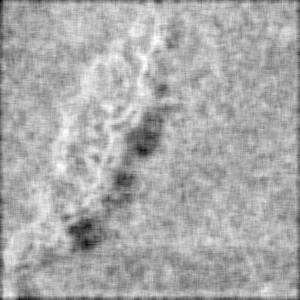
\includegraphics[keepaspectratio, width=\linewidth]{images/orig_entropy.png}
	\end{subfigure}
	\hfill
	\begin{subfigure}{0.3\linewidth}
		\centering
		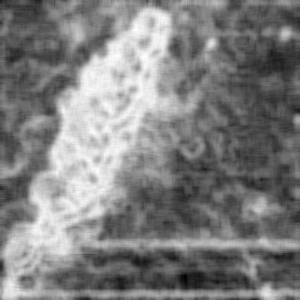
\includegraphics[keepaspectratio, width=\linewidth]{images/nlm_entropy.png}
	\end{subfigure}
	\hfill
	\begin{subfigure}{0.3\linewidth}
		\centering
		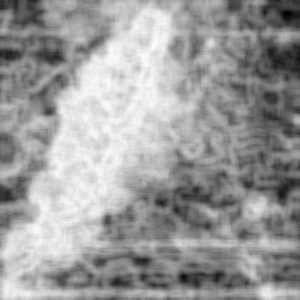
\includegraphics[keepaspectratio, width=\linewidth]{images/bm3d_entropy.png}
	\end{subfigure}\\
	\caption[Confronto delle caratteristiche dell'immagine originale con NLM e BM3D]{
		\begin{tabular}[t]{@{}l@{}}
			Confronto delle caratteristiche dell'immagine originale con \acrshort{nlm} e \acrshort{bm3d}\\
			Prima riga: Immagini\\
			Seconda riga: Mappa dell'ampiezza dei gradienti\\
			Terza riga: Rilevamento dei bordi con metodo Canny\cite{canny_1986}\\
			Quarta riga: Entropia locale dell'immagine
		\end{tabular}}
\end{figure}
\vfill
\newpage
\null
\vfill
\begin{figure}[!ht]
	\centering
	\begin{tikzpicture}
		\pgfplotstableread[col sep=comma]{data2.csv}\datatable
		
		\begin{axis}[ 
			width=7cm, height=5cm,
			legend style={legend columns=-1},
			ylabel=BRISQUE,
			xtick=data,
			xticklabels={},
			ybar,
			ymin=0,ymax=60,
			ytick={0,15,30,45,60},
			yticklabel style={
				/pgf/number format/fixed,
				/pgf/number format/precision=2
			},
			xticklabel style={rotate=90, anchor=east},
			xtick pos=bottom]
			\addplot [
			color=red,fill,
			error bars/.cd,
			y dir=both,
			y explicit,
			error bar style = {color=black, line width=1pt}
			] 
			table [x expr=\coordindex, y={meanBRISQUE}, y error={semBRISQUE}] \datatable;
		\end{axis}
		
		\begin{axis}[ 
			width=7cm, height=5cm,
			xshift=6cm,
			legend style={legend columns=-1},
			ylabel=NIQE,
			ytick pos=right,
			ylabel near ticks,
			xtick=data,
			xticklabels={},
			ybar,
			ymin=0,ymax=15,
			ytick={0,5,10,15},
			yticklabel style={
				/pgf/number format/fixed,
				/pgf/number format/precision=2
			},
			xticklabel style={rotate=90, anchor=east},
			xtick pos=bottom]
			\addplot [
			color=red,fill,
			error bars/.cd,
			y dir=both,
			y explicit,
			error bar style = {color=black, line width=1pt}
			] 
			table [x expr=\coordindex, y={meanNIQE}, y error={semNIQE}] \datatable;
		\end{axis}
		
		\begin{axis}[ 
			width=7cm, height=5cm,
			yshift=-4.5cm,
			legend style={legend columns=-1},
			ylabel=PIQE,
			xtick=data,
			xticklabels={},
			ybar,
			ymin=0,ymax=100,
			ytick={0,25,50,75,100},
			yticklabel style={
				/pgf/number format/fixed,
				/pgf/number format/precision=2
			},
			xticklabel style={rotate=90, anchor=east},
			xtick pos=bottom]
			\addplot [
			color=red,fill,
			error bars/.cd,
			y dir=both,
			y explicit,
			error bar style = {color=black, line width=1pt}
			] 
			table [x expr=\coordindex, y={meanPIQE}, y error={semPIQE}] \datatable;
		\end{axis}
		
		\begin{axis}[ 
			width=7cm, height=5cm,
			xshift=6cm, yshift=-4.5cm,
			legend style={legend columns=-1},
			ylabel=TV,
			ytick pos=right,
			xtick=data,
			xticklabels={},
			ybar,
			ymin=0,ymax=8000,
			ytick={0,2000, 4000, 6000, 8000},
			yticklabel style={
				/pgf/number format/fixed,
				/pgf/number format/precision=2
			},
			xticklabel style={rotate=90, anchor=east},
			xtick pos=bottom]
			\addplot [
			color=red,fill,
			error bars/.cd,
			y dir=both,
			y explicit,
			error bar style = {color=black, line width=1pt}
			] 
			table [x expr=\coordindex, y={meanTV}, y error={semTV}] \datatable;
		\end{axis}
		
		\begin{axis}[ 
			width=7cm, height=5cm,
			yshift=-9cm,
			legend style={legend columns=-1},
			ylabel=FSIM,
			xtick=data,
			xticklabels={},
			ybar,
			ymin=0.92,ymax=1,
			ytick={0.92,0.94,0.96,0.98,1},
			yticklabel style={
				/pgf/number format/fixed,
				/pgf/number format/precision=2
			},
			xticklabel style={rotate=90, anchor=east},
			xtick pos=bottom]
			\addplot [
			color=red,fill,
			error bars/.cd,
			y dir=both,
			y explicit,
			error bar style = {color=black, line width=1pt}
			] 
			table [x expr=\coordindex, y={meanFSIM}, y error={semFSIM}] \datatable;
		\end{axis}
		
		\begin{axis}[ 
			width=7cm, height=5cm,
			xshift=6cm, yshift=-9cm,
			legend style={legend columns=-1},
			ylabel=MI,
			ytick pos=right,
			xtick=data,
			xticklabels={},
			ybar,
			ymin=0,ymax=1,
			ytick={0,0.25,0.5,0.75,1},
			yticklabel style={
				/pgf/number format/fixed,
				/pgf/number format/precision=2
			},
			xticklabel style={rotate=90, anchor=east},
			xtick pos=bottom]
			\addplot [
			color=red,fill,
			error bars/.cd,
			y dir=both,
			y explicit,
			error bar style = {color=black, line width=1pt}
			] 
			table [x expr=\coordindex, y={meanMI}, y error={semMI}] \datatable;
		\end{axis}
		
		\begin{axis}[ 
			width=7cm, height=5cm,
			yshift=-13.5cm,
			legend style={legend columns=-1},
			ylabel=EMSE,
			xtick=data,
			xticklabels from table={\datatable}{Row},
			ybar,
			ymin=0,ymax=0.1,
			ytick={0,0.025,0.05,0.075,0.1},
			yticklabel style={
				/pgf/number format/fixed,
				/pgf/number format/precision=2
			},
			xticklabel style={rotate=90, anchor=east},
			xtick pos=bottom]
			\addplot [
			color=red,fill,
			error bars/.cd,
			y dir=both,
			y explicit,
			error bar style = {color=black, line width=1pt}
			] 
			table [x expr=\coordindex, y={meanEMSE}, y error={semEMSE}] \datatable;
		\end{axis}
		
		\begin{axis}[ 
			width=7cm, height=5cm,
			xshift=6cm, yshift=-13.5cm,
			legend style={legend columns=-1},
			ylabel=EDK,
			ytick pos=right,
			xtick=data,
			xticklabels from table={\datatable}{Row},
			ybar,
			ymin=0,ymax=0.2,
			ytick={0,0.05,0.1,0.15,0.2},
			yticklabel style={
				/pgf/number format/fixed,
				/pgf/number format/precision=2
			},
			xticklabel style={rotate=90, anchor=east},
			xtick pos=bottom]
			\addplot [
			color=red,fill,
			error bars/.cd,
			y dir=both,
			y explicit,
			error bar style = {color=black, line width=1pt}
			] 
			table [x expr=\coordindex, y={meanESI}, y error={semESI}] \datatable;
		\end{axis}
		
	\end{tikzpicture}
	\caption{Grafici a barre delle medie di valutazione per immagini O2A}
\end{figure}
\vfill
\newpage
\null
\vfill
\begin{figure}[!h]
	\centering
	\begin{tikzpicture}
		\pgfplotstableread[col sep=comma]{data3.csv}\datatable
		
			\begin{axis}[ 
				width=7cm, height=5cm,
				legend style={legend columns=-1},
				ylabel=BRISQUE,
				xtick=data,
				xticklabels={},
				ybar,
				ymin=0,ymax=60,
				ytick={0,15,30,45,60},
				yticklabel style={
					/pgf/number format/fixed,
					/pgf/number format/precision=2
				},
				xticklabel style={rotate=90, anchor=east},
				xtick pos=bottom]
				\addplot [
					color=red,fill,
					error bars/.cd,
						y dir=both,
						y explicit,
						error bar style = {color=black, line width=1pt}
				] 
				table [x expr=\coordindex, y={meanBRISQUE}, y error={semBRISQUE}] \datatable;
			\end{axis}

			\begin{axis}[ 
				width=7cm, height=5cm,
				xshift=6cm,
				legend style={legend columns=-1},
				ylabel=NIQE,
				ytick pos=right,
				ylabel near ticks,
				xtick=data,
				xticklabels={},
				ybar,
				ymin=0,ymax=15,
				ytick={0,5,10,15},
				yticklabel style={
					/pgf/number format/fixed,
					/pgf/number format/precision=2
				},
				xticklabel style={rotate=90, anchor=east},
				xtick pos=bottom]
				\addplot [
					color=red,fill,
					error bars/.cd,
						y dir=both,
						y explicit,
						error bar style = {color=black, line width=1pt}
				] 
				table [x expr=\coordindex, y={meanNIQE}, y error={semNIQE}] \datatable;
			\end{axis}
				
			\begin{axis}[ 
				width=7cm, height=5cm,
				yshift=-4.5cm,
				legend style={legend columns=-1},
				ylabel=PIQE,
				xtick=data,
				xticklabels={},
				ybar,
				ymin=0,ymax=100,
				ytick={0,25,50,75,100},
				yticklabel style={
					/pgf/number format/fixed,
					/pgf/number format/precision=2
				},
				xticklabel style={rotate=90, anchor=east},
				xtick pos=bottom]
				\addplot [
					color=red,fill,
					error bars/.cd,
						y dir=both,
						y explicit,
						error bar style = {color=black, line width=1pt}
				] 
				table [x expr=\coordindex, y={meanPIQE}, y error={semPIQE}] \datatable;
			\end{axis}
			
			\begin{axis}[ 
				width=7cm, height=5cm,
				xshift=6cm, yshift=-4.5cm,
				legend style={legend columns=-1},
				ylabel=TV,
				ytick pos=right,
				xtick=data,
				xticklabels={},
				ybar,
				ymin=0,ymax=8000,
				ytick={0,2000, 4000, 6000, 8000},
				yticklabel style={
					/pgf/number format/fixed,
					/pgf/number format/precision=2
				},
				xticklabel style={rotate=90, anchor=east},
				xtick pos=bottom]
				\addplot [
					color=red,fill,
					error bars/.cd,
						y dir=both,
						y explicit,
						error bar style = {color=black, line width=1pt}
				] 
				table [x expr=\coordindex, y={meanTV}, y error={semTV}] \datatable;
			\end{axis}
		
			\begin{axis}[ 
				width=7cm, height=5cm,
				yshift=-9cm,
				legend style={legend columns=-1},
				ylabel=FSIM,
				xtick=data,
				xticklabels={},
				ybar,
				ymin=0.92,ymax=1,
				ytick={0.92,0.94,0.96,0.98,1},
				yticklabel style={
					/pgf/number format/fixed,
					/pgf/number format/precision=2
				},
				xticklabel style={rotate=90, anchor=east},
				xtick pos=bottom]
				\addplot [
					color=red,fill,
					error bars/.cd,
						y dir=both,
						y explicit,
						error bar style = {color=black, line width=1pt}
				] 
				table [x expr=\coordindex, y={meanFSIM}, y error={semFSIM}] \datatable;
			\end{axis}
			
			\begin{axis}[ 
				width=7cm, height=5cm,
				xshift=6cm, yshift=-9cm,
				legend style={legend columns=-1},
				ylabel=MI,
				ytick pos=right,
				xtick=data,
				xticklabels={},
				ybar,
				ymin=0,ymax=1,
				ytick={0,0.25,0.5,0.75,1},
				yticklabel style={
					/pgf/number format/fixed,
					/pgf/number format/precision=2
				},
				xticklabel style={rotate=90, anchor=east},
				xtick pos=bottom]
				\addplot [
					color=red,fill,
					error bars/.cd,
						y dir=both,
						y explicit,
						error bar style = {color=black, line width=1pt}
				] 
				table [x expr=\coordindex, y={meanMI}, y error={semMI}] \datatable;
			\end{axis}

			\begin{axis}[ 
				width=7cm, height=5cm,
				yshift=-13.5cm,
				legend style={legend columns=-1},
				ylabel=EMSE,
				xtick=data,
				xticklabels from table={\datatable}{Row},
				ybar,
				ymin=0,ymax=0.1,
				ytick={0,0.025,0.05,0.075,0.1},
				yticklabel style={
					/pgf/number format/fixed,
					/pgf/number format/precision=2
				},
				xticklabel style={rotate=90, anchor=east},
				xtick pos=bottom]
				\addplot [
					color=red,fill,
					error bars/.cd,
						y dir=both,
						y explicit,
						error bar style = {color=black, line width=1pt}
				] 
				table [x expr=\coordindex, y={meanEMSE}, y error={semEMSE}] \datatable;
			\end{axis}
			
			\begin{axis}[ 
				width=7cm, height=5cm,
				xshift=6cm, yshift=-13.5cm,
				legend style={legend columns=-1},
				ylabel=EDK,
				ytick pos=right,
				xtick=data,
				xticklabels from table={\datatable}{Row},
				ybar,
				ymin=0,ymax=0.2,
				ytick={0,0.05,0.1,0.15,0.2},
				yticklabel style={
					/pgf/number format/fixed,
					/pgf/number format/precision=2
				},
				xticklabel style={rotate=90, anchor=east},
				xtick pos=bottom]
				\addplot [
					color=red,fill,
					error bars/.cd,
						y dir=both,
						y explicit,
						error bar style = {color=black, line width=1pt}
				] 
				table [x expr=\coordindex, y={meanESI}, y error={semESI}] \datatable;
			\end{axis}
						
	\end{tikzpicture}
	\caption{Grafici a barre delle medie di valutazione per immagini O3A}
\end{figure}
\vfill
\newpage 

\section{Ispezione visiva multicanale}

L'ispezione visiva può essere anche eseguita utilizzando l'immagine dell'ampiezza \acrshort{snom} in combinazione con l'immagine di topografia e fase \acrshort{snom} per verificare la correlazione delle caratteristiche nelle immagini. L'immagine di topografia è posta nel canale rosso, quella dell'ampiezza \acrshort{snom} nel canale verde e infine quella della fase \acrshort{snom} nel canale blu.\\

\begin{figure}[h]
	\centering
	\begin{subfigure}{0.32\linewidth}
		\centering
		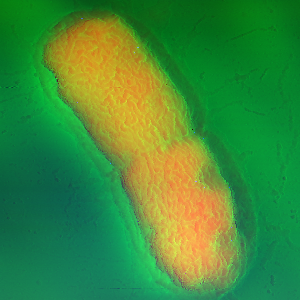
\includegraphics[keepaspectratio, width=\linewidth]{images/multi_orig.png}
		\caption{Originale}
	\end{subfigure}
	\begin{subfigure}{0.32\linewidth}
		\centering
		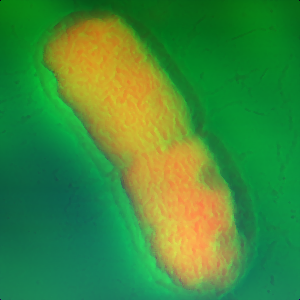
\includegraphics[keepaspectratio, width=\linewidth]{images/multi_med.png}
		\caption{Mediana}
	\end{subfigure}
	\begin{subfigure}{0.32\linewidth}
		\centering
		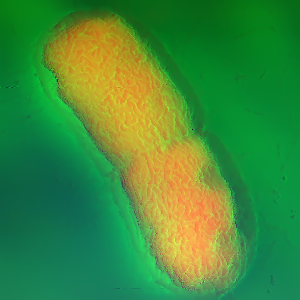
\includegraphics[keepaspectratio, width=\linewidth]{images/multi_nlm.png}
		\caption{NLM}
	\end{subfigure}
	\caption{Ispezione visiva multicanale di un'immagine della $2^a$ armonica}
\end{figure} 

Si può notare come il filtro mediana abbia rimosso il rumore impulsivo presente soprattutto sui bordi del batterio preservando comunque dei bordi definiti, ma sono diminuiti i dettagli delle strutture interne. Al contrario, il filtro NLM ha preservato i bordi e i dettagli del campione ma non è riuscito a rimuovere il rumore impulsivo sui bordi. Tuttavia, ha svolto un lavoro nettamente migliore nel rimuovere le imperfezioni sul piano di osservazione lasciando però inalterato il batterio.

\section{Analisi correlativa}
La microscopia \acrshort{ssnom} ha suscitato interesse negli ultimi anni, ma il suo impiego nella \gls{microbiologia} è rimasto limitato, soprattutto per le difficoltà nell'interpretare i dati a causa della scarsa disponibilità dei dati. Come accennato in precedenza, un microscopio può offrire più tecniche di microscopia per studiare più proprietà dello stesso materiale nello stesso momento, per questo recenti studi hanno accoppiato un sistema di microscopia \acrshort{ssnom} ad altri sistemi per avere un contesto noto per analizzare i dati provenienti dal campo vicino, come la microscopia \acrfull{afm} o \acrshort{clsm}.\cite{stanciu_2017}\\

\begin{figure}[h]
	\centering
	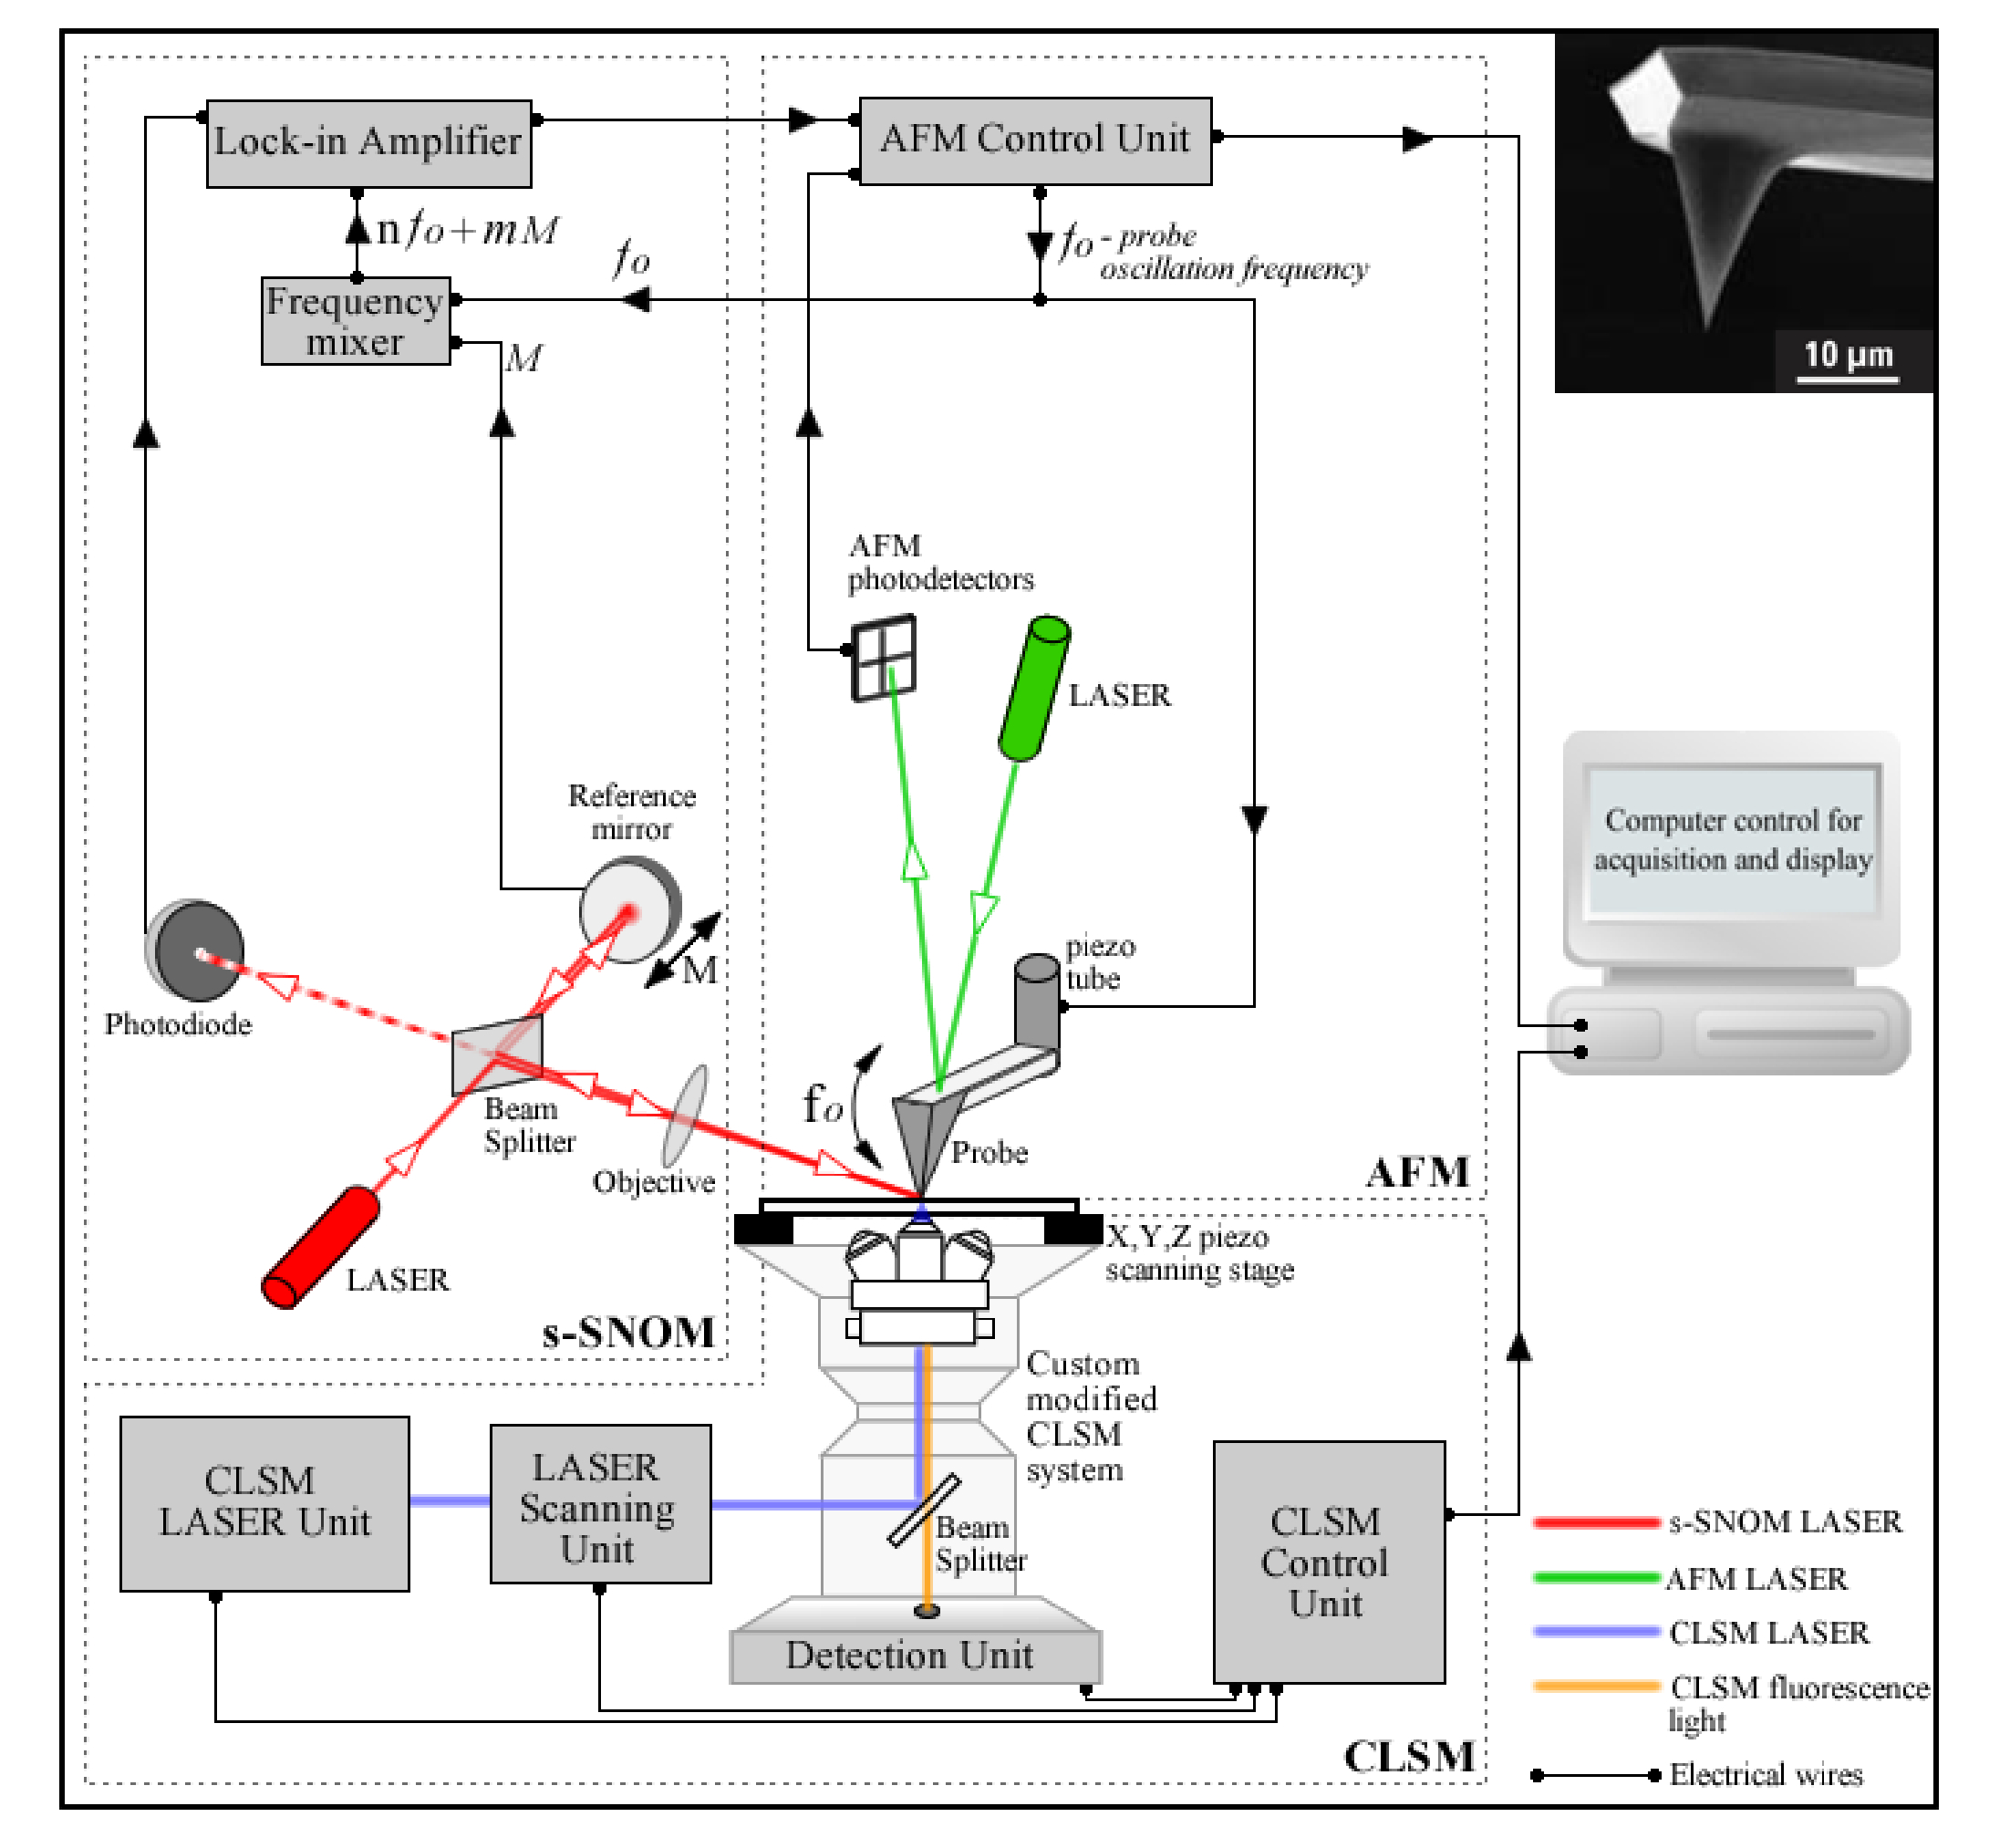
\includegraphics[keepaspectratio, height=\linewidth]{images/multimodal_system.jpg}
	\caption[Sistema multimodale per l'acquisizione di immagini correlative]{
		Sistema multimodale per l'acquisizione di immagini correlative \cite{stanciu_2017}}
	\label{fig:multimodal_system}
\end{figure}

\end{document}